

\begin{abstract}
    Seismic fragility curves are key quantities of interest in the seismic probabilistic risk assessment framework because they efficiently describe the fragility of a mechanical system of interest under a seismic excitation. They are studied since the 1980s on various types of data and characterization of the seismic motion and of the structure's response. 
    In this chapter, we propose a review of the numerous methods that exist to estimate the curves. We particularly describe the role played by the characteristics of the available data to select a modeling of the fragility curve.
    This chapter is also the occasion to present some mechanical equipments that will be studied in the following chapters of this manuscript.
\end{abstract}

\minitoc


\section{Introduction}

% The SPRA contains several tools and things

The Seismic Probabilistic Risk Assessment (SPRA) defines a framework and a methodology for the study of seismic structural reliability. %This framework is parrt of the probabilistic 
% As for the Pr
It has been introduced since 1968 \citep{cornell_engineering_1968}
to incorporate the seismic risk evaluation in the probabilistic risk assessment studies.
% and further developed in the
The SPRA has been mostly developed and carried out in the 1980s on nuclear facilities (see e.g. \cite{kennedy_probabilistic_1980,kennedy_seismic_1984}). 
It includes: the determination of the seismic hazard, the analysis of the seismic fragility of structural components, the evaluation of the risks combination and their consequences in the system, as described in the report of the Electric Power Research Institute \citep{epri_seismic_2013}, which provides guidelines for its implementation. %among other ingredients.
%The guidelines for its implementation are thoroughly described in the 
It is since widely used in the nuclear industry (e.g. \cite{ellingwood_validation_1990,park_survey_1998,kennedy_risk_1999}) and its consideration is established among the safety standards adopted by the International Atomic Energy Agency \citep{iaea_probabilistic_2020}.

% Estimating th

Within the SPRA, seismic fragility curves represent a key asset that play a prominent role in the analysis of structural components' fragility step (see  \cite{epri_advanced_2011}).
They express in probabilistic terms the fragility of structures under seismic excitation. We can mention that they are also a tool of interest of performance-based earthquake engineering (PBEE; \cite{ghobarah_performance-based_2001,noh_development_2014}), 
which aims at relating performance objectives to level of damage to the structure.
In any case, they are defined as a function of the seismic hazard, which ---driven by the magnitude (M), the source-site distance (R), and other earthquake parameters--- is reduced to a scalar value derived from the seismic signal: the intensity measure (IM), under the so-called ``sufficiency assumption'' \citep{cornell_hazard_2004,luco_structure-specific_2007}.
In practice, a fragility curve, denoted $P_f$, therefore expresses the probability of failure of a mechanical structure as a function of an IM value of interest such as peak ground acceleration (PGA) or pseudo-spectral acceleration (PSA), among others:
    \begin{equation}
        P_f(a) = \PP(\text{``failure''}|\text{IM}=a).
    \end{equation}
Within the SPRA framework, the fragility curve expression is expected to be combined with the seismic hazard frequency to compute the  annual damage frequency of the component $C_f$:
    \begin{equation}\label{eq:intro-frags:damagefrequency}
        C_f =  \int_0^\infty P_f(a)\left|dH(a)\right|.
    \end{equation}
Here, $|dH(a)|=|\frac{d}{da}\PP(\text{IM}>a)|da$ is defined from the mean annual  frequency of exceedance of a ground motion of level $a$. %,then $C_f$ represents the annual damage frequency of the component. 
To derive the damage frequency $C_f$, seismologists determine $|dH|$ using not only records of seismic signals but also historical data, geological information, and geotechnical analysis.
%  beyond accelerogram records (e.g., ).
It should be noted that the sufficiency assumption was introduced to reduce estimation costs since it assumes that the fragility curve of a given structure is identical regardless of the seismic scenario.
Actually, this assumption embeds some uncertainty in the problem since, as shown in \citeauthor{radu_earthquake-source-based_2018}, \citeyearlink{radu_earthquake-source-based_2018,grigoriu_are_2021}, %\cite{radu_earthquake-source-based_2018,grigoriu_are_2021}, 
different seismic scenarios can lead to identical distributions of some IMs, although the underlying seismic signals have significantly different frequency contents.
The uncertainty rooted in the fragility curve by this assertion could be classified as an \emph{aleatoric} (irreducible) kind of uncertainty
 (we refer to \cref{chap:intro-english} for the definition of the uncertainty quantification framework).
% belong to the category of
%The evaluation of the fragility curve defined in eq  implies the consideration of this
% Focusing the definition of the fragility curve <


In this second part of the manuscript, we focus on the estimation of seismic fragility curves. 
Thus, we do not address the determination of the seismic hazard $H$, which is the responsibility of seismologists, 
%question the determination of the seismic hazard distribution $H$, 
nor the derivation of the damage frequency of the component $C_f$.
Nevertheless, estimating the fragility curve itself %for given mechanical equipment 
remains a daunting task. It is commonly done statistically, using different kind of methods depending 
on the source of data available, their characteristics, and their quantity.
This chapter proposes a review of these methods. 
In the next section,
we define the different kind of data involved when estimating seismic fragility curves. In particular, we present a stochastic seismic signal generator, and  we present how the failure of mechanical equipment is generally defined.
In \cref{sec:intro-frags:models}, different models and methods are presented, they are grouped in two categories: the non-parametric ones and the parametric ones.
Explicit examples of case studies are then given in \cref{sec:intro-frags:casstudies}, from a theoretical one to an experimental one for which really few data are available.
%Given those and the non-exhaustive list of modeling we present from the literature, we question 
Conclusive thoughts are proposed in \cref{sec:intro-frags:conclusion}.






% steps of seismic hzarad determination or r
% The derivation 




% it embedds uncertainty suinc...

% that in the step
%As shown in \cite{Radu2018,Grigoriu2021}, different seismic scenarios can however lead to identical distributions of some IMs, although the underlying seismic signals have significantly different frequency contents. As a result, the sufficiency assumption is not met, especially for non-linear, multimodal structures, etc., with current IMs. 
%
%
% Despite this, it is possible to focus on the definition of the resulting fragility curve, without taking the assumption for granted, which is the case in this work.

% and is widely used in in the nuclear industry







% Seismic fragility curves represent a key one. They were introduced in the 1980s for seismic risk assessment studies carried out on nuclear facilities \citep{kennedy_probabilistic_1980,kennedy_seismic_1984,ellingwood_validation_1990,park_survey_1998,kennedy_risk_1999,cornell_hazard_2004}.


% %IN the SPRA, historic, lot of things are defined,
% %among them, the seismic fragility curves. 
% %They represent an essential tool..
% Also used in PBEE, link with insurance?

% IM, sufficientcy assumption. Different, various scenario and methods
% Quantification of uncertainty?


% This chapter suggests a review of the main methods that exist in the literature 




\section{Data: from seismic signals to equipments failures}\label{sec:intro-frags:data}





In the literature, different sources of data are exploited to estimate seismic fragility curves. 
We can cite, for instance:
(i) expert assessments supported by test data (e.g. \cite{kennedy_probabilistic_1980,kennedy_seismic_1984,zentner_fragility_2017}), (ii) experimental data (e.g. \cite{park_survey_1998}), (iii) empirical data from past earthquakes (e.g. \cite{shinozuka_statistical_2000,straub_improved_2008,lallemant_statistical_2015,buratti_empirical_2017,laguerre_empirical_2024}), and (iv) analytical results obtained from various numerical models using artificial or natural seismic excitations (e.g. \cite{ellingwood_earthquake_2001,kim_development_2004,zentner_numerical_2010,koutsourelakis_assessing_2010,mai_seismic_2017,trevlopoulos_parametric_2019,wang_influence_2020,mandal_seismic_2016,wang_seismic_2018,wang_bayesian_2018,zhao_seismic_2020,katayama_bayesian-estimation-based_2021,gauchy_importance_2021,khansefid_fragility_2023,lee_efficient_2023}).
In every of these studies, each sample in 
the dataset regroups:
\begin{enumerate}
    \item Information about a seismic ground motion. The considered ground motions are sometimes natural and sometimes artificial. The information can take several forms, %(such as the temporal signal), 
    as stated in the introduction it is generally used  to derive one or several scalars called intensity measures (IMs).
    % as stated in the introduction, it is generally used to 
    \item Information about the response of the structure or the equipment of interest to the seismic excitation. To define the fragility curve, this information, must permit to characterize the failure of the studied system.
\end{enumerate}
%(i) information about the seismic ground motion (it can be the temporal signal itself,)

% In the subsection   we pre



Since available records of real seismic excitations for a given site are often scarce, it is common to construct a dataset of artificial earthquake accelerograms using a seismic signal generator.
Various techniques exist for this purpose. According to \citet{rezaeian_stochastic_2008}, the methods can be categorized among the ``source-based'' ones, which model the occurrence of
earthquake rupture at some sources and the propagation of seismic waves to the studied site, and the ``site-based'' ones, which model the seismic signals for the site of interest from the consideration of its characteristics and historical recorded earthquakes.
A review of the first kind is proposed in \cite{zerva_seismic_1988}, and a review of the second can be found in \cite{shinozuka_stochastic_1988}.
As more recent examples for the latter, we can also cite \cite{trevlopoulos_parametric_2019}; and \cite{zentner_enrichment_2012}.
In the following, we present a stochastic seismic signal generator that is proposed by \citet{rezaeian_simulation_2010}. It lies among the site-based models, and has been implemented by \citet{sainct_efficient_2020}, who calibrated it using $97$ real accelerograms selected in the European Strong Motion Database  for a magnitude $M$ such that $5.5 \leq M \leq 6.5$, and a source-to-site distance $R < 20$~km \citep{ambraseys_dissemination_2000}.  An example of one of these real signals is plotted in 
\cref{fig:intro-frags:real-seism}.




As said in the introduction, this thesis does not seek to question thoroughly the seismic hazard, and we aim at providing methods that can be applied to any modeling of the seismic signals. Nevertheless, in the following chapters, our methods are applied and validated on different case studies that are presented later on. These case studies take the form of mechanical equipments that have been submitted to artificial seismic signals generated using the generator implemented by \citet{sainct_efficient_2020}, and presented below.


\begin{figure}[h]
    \centering
    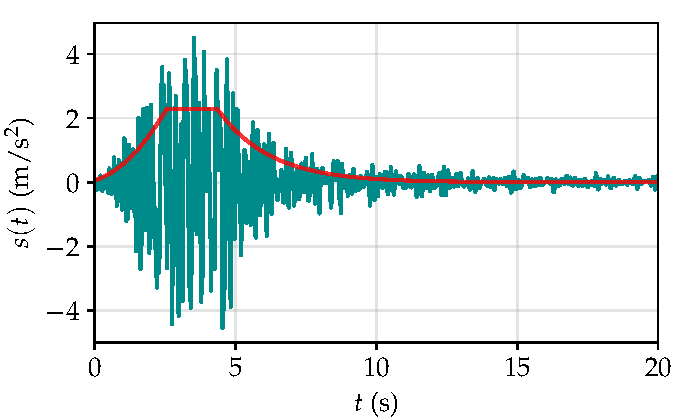
\includegraphics[width=5.625cm]{figures/intro-frags/seism1.pdf}\hspace*{0.5cm}
    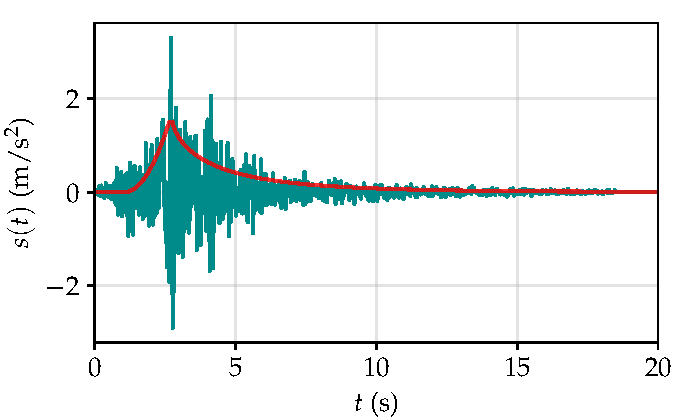
\includegraphics[width=5.625cm]{figures/intro-frags/seism2.pdf}
    \caption{Example of two accelerogram records of real seismic signals (cyan). For each signal, its envelope $q(t,\boldsymbol{\rho})$ is plotted in red.} %: the realtive acceleration $s$ of the ground is .}
    \label{fig:intro-frags:real-seism}
\end{figure}


%the case studies that we present and onto which we will apply our methods are excited using



\subsubsection{Seismic signals generator and IMs}


The generator model a seismic excitation as a temporal signal that is the realization
$s:t\in[0,T]\mapsto s(t)\in\RR$ of a random process defined on a probability space $(\Omega,\Xi,\PP)$. 
The process presented here corresponds to a filtered stochastic white noise with time dependent parameters:
    \begin{equation}\label{eq:intro-frags:sgenertor}
        s(t)= s(t;w,\boldsymbol{\rho},\boldsymbol{\lambda}) = q(t,\boldsymbol\rho)\left[\frac{1}{\sigma_f(t)}\int_{-\infty}^t h_f(t-\tau,\boldsymbol\lambda)w(\tau)d\tau \right],
    \end{equation}
where $w$ is a realization of a Gaussian white noise process $W$. In other terms $W:[0,T]\times\Omega\to\RR$ is such that for all $t_1<t_2$, $t_3<t_4$, 
$\int_{t_1}^{t_2}W(\tau)d\tau\sim\cN(0,(t_2-t_1)\sigma^2)$, and $\EE\int_{t_1}^{t_2}W(\tau)d\tau\int_{t_3}^{t_4}W(\tau)d\tau=(\min(t_2,t_4)-\max(t_1,t_3))^+\sigma^2$.

% $\EE W(t_1)=0$, $\EE W(t_1)^2=\infty$, and $\EE W(t_1)W(t_2)=0$.

The integral in \cref{eq:intro-frags:sgenertor} corresponds to the filtering of $w$, $h_f(t,\boldsymbol{\lambda})$ being the impulse response function (IRF) of the linear filter and $\sigma_f^2$ being its variance: $\sigma_f^2(t)=\int_{-\infty}^th^2(t-\tau,\boldsymbol{\lambda}(\tau))d\tau$. The IRF is defined by
    \begin{equation}
        h_f(t-\tau,\boldsymbol{\lambda}) = \frac{\omega_f(\tau)}{\sqrt{1-\zeta^2_f}}\exp[-\zeta_f\omega_f(\tau)(t-\tau)]\sin\left(\omega_f(\tau)\sqrt{1-\zeta^2_f}(t-\tau)\right)\indic_{t\geq\tau},
    \end{equation}
with $\omega_f(\tau):=\omega_0+\frac{\tau}{T}(\omega_n-\omega_0)$. 
The IRF $h_f$ corresponds to the response of a linear oscillator with damping ratio $\zeta_f$ and time-dependent natural frequency $\omega_f(\tau)$. It is parameterized by $\boldsymbol{\lambda}=(\omega_0,\omega_n,\zeta_f)\in(0,\infty)^2\times[0,1]$.




% with $\boldsymbol{\lambda}(\tau)=(\omega_0,\omega_n\zeta_f) $ where $\omega_f(\tau):=\omega_0+\frac{\tau}{T}(\omega_n-\omega_0)$ being the natural frequency and $\zeta_f\in[0,1]$ being a constant damping ratio. 
% The quantities $\omega_0$ and $\omega_n$ are parameters of the IRF.

 The function $q(t,\boldsymbol\rho)$ is a
 non-negative modulating function that represents the envelope of the accelerogram, it is defined by
    \begin{equation}
        q(t,\boldsymbol\rho) = \left\lbrace \begin{array}{ll}
            \rho_1t^2/T_1^2 & \text{if\ } 0\leq t< T_1 \\
            \rho_1 & \text{if\ }T_1\leq t< T_2\\
            \rho_1\exp\left[-\rho_2(t-T_2)^{\rho_3}\right] &\text{if\ }T_2\leq t
        \end{array}\right.
    \end{equation}
where $\boldsymbol\rho=(\rho_1,\rho_2,\rho_3,T_1,T_2)\in(0,\infty)^5$.


%For each of the seimsic records 
%As previously announced, 
%Given an accelerogram record $\tilde s$, 
A real accelerogram record is associated to parameters $(\boldsymbol{\lambda},\boldsymbol{\rho})$ by conducting signal processing techniques. We refer to \cite{rezaeian_stochastic_2008} for more details.
In \cref{fig:intro-frags:real-seism}, the envelopes $q(\cdot,\boldsymbol{\rho})$ associated with two real seismic signals are plotted.
As previously announced,
we consider $N_r=97$ real acceleration records form the European Strong Motion Database for a magnitude $M$ such that $5.5\leq M\leq 6.5$ and a source-to-site distance $R<20$~km. They have been associated to parameters $\overline{\boldsymbol{\phi}}_i:=(\overline{\boldsymbol{\lambda}}_i,\overline{\boldsymbol{\rho}}_i)$, $i=1,\dots,N_r$.



To generate artificial seismic signals, we propose sampling realizations of the process $s(\cdot;W,\boldsymbol{\phi})$, where $\boldsymbol{\phi}\in\mbf D:=(0,\infty)^7\times[0,1]$ is stochastic and follows a distribution that corresponds to the empirical distribution of the $(\overline{\boldsymbol{\phi}}_i)_{i=1}^{N_r}$. More precisely, the distribution of $\boldsymbol{\phi}$ is  given by the Gaussian kernel density estimation %(see \cite{kristan_multivariate_2011}) 
of the one of the $(\overline{\boldsymbol\phi}_i)_{i=1}^{N_r}$, i.e., its density $p_{\boldsymbol{\phi}}$ is given by
\begin{equation}
    p_{\boldsymbol{\phi}}(x) \propto \sum_{i=1}^{N_r}\exp\left( -\frac{1}{2} (x-\overline{\boldsymbol\phi}_i)^\top\Sigma^{-1}(x-\overline{\boldsymbol\phi}_i) \right)\indic_{x\in\mbf D},
\end{equation}
where $\Sigma$ is derived from the $(\overline{\boldsymbol{\phi}}_i)_{i=1}^{N_r}$ (see \cite{kristan_multivariate_2011}).

To sample from the generator, a tuple of parameters $\tilde{\boldsymbol{\phi}}$ is sampled given the distribution of $\boldsymbol{\phi}$. Then, the filtered Gaussian noise is approximated by a truncation of the integral in \cref{eq:intro-frags:sgenertor}:
    \begin{equation}
        \int_{-\infty}^t h_f(t-\tau,\boldsymbol\lambda)W(\tau)d\tau \approx \sum_{j=0}^{M}h_f(t- \tau(j),\boldsymbol{\lambda} ) \int_{\tau(j)}^{\tau(j+1)}W(\tau)d\tau, %,\quad \tau(j) = -M_2+ \frac{j(t+M_2)}{M_1}, %j(t+M_2)/M_1
    \end{equation}
where $\tau(0),\dots,\tau(M)$ is a subdivision of a subset of $(-\infty,t)$.
The above approximation can be sampled using $\int_{\tau(j)}^{\tau(j+1)}W(\tau)d\tau\sim\cN(0,(\tau(j+1)-\tau(j))\sigma^2)$.





% As previously announced,
% the records considered are $N_r=97$ real acceleration records form the European Strong Motion Database for a magnitude $M$ such that $5.5\leq M\leq 6.5$ and a source-to-site distance $R<20$~km.
% Therefore, the signal $s$ depends on $w$ and 
% $\boldsymbol{\phi}:=(\boldsymbol{\rho},\omega_0,\omega_n,\zeta_f)\in\boldsymbol{\Phi}:=(0,\infty)^7\times[0,1]$.
% The generator consists in deriving realizations of $s(\cdot;W,\boldsymbol\phi)$ where 
% $\boldsymbol{\phi}$
% is stochastic,
% its distribution being identified using real acceleration records.
% As previously announced,
% the records considered are $N_r=97$ real acceleration records form the European Strong Motion Database for a magnitude $M$ such that $5.5\leq M\leq 6.5$ and a source-to-site distance $R<20$~km.
% Each of the records corresponds to a realization of $s(\cdot;W,\overline{\boldsymbol{\phi}}_i)$ using a tuple $\overline{\boldsymbol\phi}_i$ as parameters. The distribution of $\boldsymbol{\phi}$ 


From a seismic signal $s$ that is a realization of the process described above, different intensity measure  indicators can be derived.
The choice of the appropriate IM to estimate seismic fragility curves
remains a complex question. 
According to \citet{giovenale_comparing_2004}, the appropriateness of an IM must be defined in terms of efficiency, sufficiency, and hazard compatibility.
However, the most efficient or sufficient IM is not the same for two different case studies (see \cite{mackie_probabilistic_2001,hariri-ardebili_probabilistic_2016}). % changes when a different case 
%regarding the studied system, the results given
% study is considered (see ). 
Moreover, while we do not  thoroughly research the best IM in this thesis, we will see in the following chapters that the best choice is not necessarily simply the one that is the most correlated with the structure's response.
Below we propose a non-exhaustive list of common IMs, a more complete one can be found in \cite{luco_structure-specific_2007}:
    \begin{itemize}
        \item the peak ground acceleration (PGA) is defined as $\text{PGA}=\max_{t\in[0,T]}|s(t)|$;
        \item the peak ground velocity (PGV) is defined as $\text{PGV}=\max_{t\in[0,T]}\left|\int_0^ts(\tau)d\tau \right|$;
        \item the peak ground displacement (PGD) is defined as $\text{PGD}=\max_{t\in[0,T]}\left|\int_{0}^{t}\int_{0}^{\tau}s(u)dud\tau\right|$;
        \item the pseudo spectral acceleration (PSA) at frequency $f_L$ and damping ratio $\xi$ is defined as $\text{PSA}=(2\pi f_L)^2\max_{t\in[0,T]}|x(t)|$, where $x$ is the solution of the linear equation
        \begin{equation}\label{eq:intro-frag:ALS}
            x''(t) + 2\xi2\pi f_Lx'(t)+(2\pi f_L)^2x(t) = -s(t).
        \end{equation}
        This IM is component-dependent since, in practice, the damping ratio $\xi$ and the frequency $f_L$ are evaluated from the mechanical characteristic of the studied system. Generally, the frequency $f_L$ considered for deriving the PSA corresponds to the first mode of the structure's response under excitation. \Cref{eq:intro-frag:ALS} corresponds to the response equation of the linear single degree of freedom system associated to the structure.
    \end{itemize}

For  conducting the numerical experiments of this thesis, $10^5$ seismic signals have been computed using this generator.
In \cref{fig:intro-frags:IM-density}, we draw the distribution of the PGA and the PSA (at frequency $5$~Hz and damping ratio $1\%$) given by this generator. It is compared with the kernel density approximation of the PGA and PSA values of the $97$ real seismic signals that have been used for fitting the generator. %, and with a lognormal distribution with same median and same log deviation. 
These comparisons show that the synthetic signals have realistic features.
It is important to note, that the distribution of the IM produced by this generator may differ in practice from the distribution used to derive the damage frequency evoked in \cref{eq:intro-frags:damagefrequency}. The latter is typically based on a more comprehensive characterization of the IM, incorporating not only recorded signals but also additional sources such as historical data, geological information, and geotechnical analyses.


% We precise here that the distribution of the IM given by this generator may differ in practice from the one used to derive the damage frequency evoked in \cref{eq:intro-frags:damagefrequency}. Indeed, the latter is derived using a distribution of the IM that is determined by richer sources on top of signal records. % a more rich analysi
%hazard 


\begin{figure}[h]
    \centering
    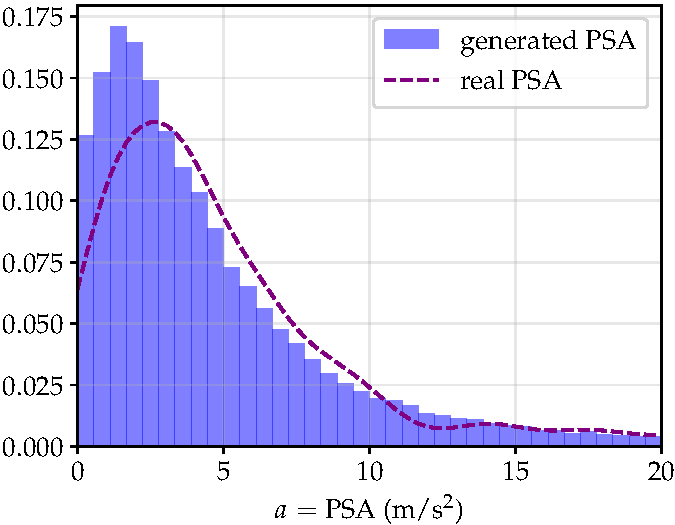
\includegraphics[width=5cm]{figures/intro-frags/PSA_density.pdf}\ 
    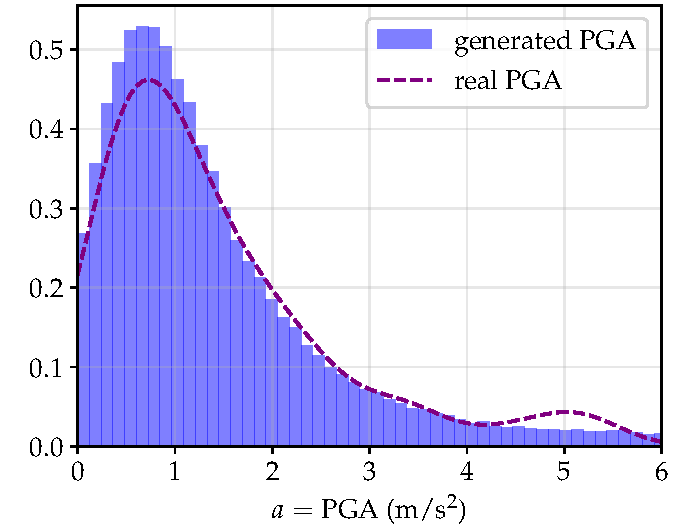
\includegraphics[width=5cm]{figures/intro-frags/PGA_density.pdf}
    \caption{Histograms of IMs derived from $10^5$ generated synthetic signals : the IM is the PSA (left) and the PGA (right). They are compared with the densities of IMs coming from real accelerograms estimated by Gaussian kernel estimation (dashed lines).} %, {and with the densities of a lognormal distribution with same median and same log deviation (solid lines).}}
    \label{fig:intro-frags:IM-density}
\end{figure}



 %the conduction of 
%  the numerical experiments conducted 



%different IMs


% Regarding seismic ground motions, a common methodology



% SAinct et al

% definition of IMs


\subsubsection{Engineering demand parameter and failure}


As evoked in the preamble of this section, numerous data sources exist for identifying the fragility (and the failure) of mechanical structures and components.
In most cases a particular engineering demand parameter (EDP) of the system is focused on. The EDP is a scalar quantity that is observed (numerically or practically) during the seismic excitation, it can be the maximal displacement of a specific part of mechanical equipment for instance. More explicit examples will be given when specific case studies will be presented later on in this chapter. 
In those cases, the failure is defined when the EDP exceeds a threshold limit.

All in all, available datasets often take the form of tuples $((\cS_i,\cD_i))_{i=1}^k$, where $\cS_i$ is the $i$-th seismic signal submitted to the system and $\cD_i$ is the EDP that was observed during the experiment. %The reduced 
%
In the case studies that are treated in this manuscript a specific IM is chosen, and a reduced dataset of the form $((a_i,z_i))_{i=1}^k$ is studied, where $a_i$ is the IM of the $i$-th seismic signal, and $z_i=\indic_{\cD_i> C }$, where $ C $ is the threshold that defines the failure of the system. In other words, $z_i=1$ if the system has failed when submitted to the  $i$-th seismic signal, and $z_i=0$ otherwise.
The dataset permits to statistically estimate the fragility curve of the system of interest. In this thesis, we restrict the study to cases where the observations can be considered independent. 
Naturally, this restriction excludes certain case studies, such as experimental campaigns carried out on certain structures subjected to a series of seismic solicitations of increasing level, such as reinforced concrete structures, because these systems are damaged with each seismic solicitation.
%
%Naturally, that restriction excludes some case studies, such as experimental campaigns conducted on concrete structures for instance, since such systems get damaged during the experiment, impacting their mechanical behavior. 
The advantage of considering binary data (failure or non-failure) is that it allows to deal with cases for which (i) the failure is defined by multiple criteria (e.g. stacked structures) and (ii) an EDP is not directly observed (e.g. electrical devices).

%As mechanical systems that enter the scope of this thesis, we can cite
%\begin{itemize}
    % \item 
%    structures and component  whose response under seismic excitation can be modeled numerically (via finite element analysis for instance), and
    % \item 
%    sturdy mechanical equipments that do not get damaged during experimental campaigns such as pipes, electronic devices, stacked structures.
%\end{itemize}
%In the last two examples evoked, the failure is not always characterized by observing an EDP, and can be multifactorial. While the studies that are done in this thesis are limited to cases where the system of interest's failure is characterized by an EDP, we emphasize that the methods that we develop and use go beyond these specific cases.



% However, structures and components whose response under seismic excitation can be modeled numerically via finite element methods are


% various mechanical equipment in the nuclear industry are sturdy enough 






\section{Modeling of the fragility curve}\label{sec:intro-frags:models}

Different models and methods have been suggested in the literature to estimate seismic fragility curves.
%Historically, the 
In the genesis of the SPRA, seismic fragility curves were estimated based on expert judgments, principally due to the scarcity of available data to conduct an accurate statistical estimation (see \cite{kennedy_probabilistic_1980}).
Of course, the accuracy of such an estimation is not guaranteed either, and its reliability depends on that of the experts.

Nowadays, estimates of seismic fragility curves are mostly derived using statistical techniques, leveraging (i) dataset that are sometimes less scarce and more precise, and also (ii) statistical techniques that are more efficient. 
The expert judgment still complement those in some works in the literature.


Non-parametric and parametric methods are both used in the literature to estimate seismic fragility curves.
In the former, the probabilistic relation between the failure and the IM is sought. When an EDP is available, authors seek to estimate first the probabilistic relation between the IM and the EDP, to deduce the resulting fragility curve.
In the latter, the fragility curve is assumed to belong to a parameterized set, reducing the problem to the estimation of these parameters.
While the first method is more general in the sense that it covers a wider range of possible estimates, it is also often less efficient than the second. Indeed, reducing the problem to a finite-dimensional one allows providing satisfying estimates with fewer data. However, their reliability depends on the trustworthiness of the chosen parametric modeling.

In the following, we review briefly the
state-of-the art on the estimation of seismic fragility curves. We start by a review of non-parametric methods in \cref{sec:intro-frags:subsec-nonparametric}. In that section we also describe a non-parametric estimation that is based on Monte-Carlo estimates, and that can serve as a reference when a large dataset is available.
In \cref{sec:intro-frags:subsec-parametric} we discuss the parametric modelings of the fragility curves, and we present the most common one: the probit-lognormal model.



% , in which we p



% Two main different approaches exist to model the fragility curve. Firstly, one approach consists in estimating 
% It is common to classify the modelings of fragility curves in two categories: the non-parametric ones and the pa








%\subsection{A state-of-the-art}





\subsection{Non-parametric modeling}\label{sec:intro-frags:subsec-nonparametric}


Most of non-parametric models for seismic fragility curves estimation leverage ---if possible--- the knowledge of an EDP that describes more precisely the response of the structure under seismic excitation than just the binary outcome ---failure or non-failure.
In this case it is possible to estimate the conditional distribution of the EDP to the IM (or IMs) via a surrogate modeling of the system $\text{EDP}=\cM(\text{IM})$.

Among common surrogates we can mention the Gaussian processes (GPs). As examples of their use for seismic fragility curves estimation, we can cite \cite{gidaris_kriging_2015}, in which GPs are used to estimate the EDP given multiple parameters characterizing the ground motion; and \cite{gauchy_uncertainty_2024}, in which the GPs-based estimation of the EDP is coupled with a sensitivity analysis of the fragility curve to the mechanical parameters of the studied system.

We also mention polynomial chaos expansion (PCE) as a surrogate numerously used for seismic fragility curves estimation. For instance, PCEs are combined in \cite{mai_surrogate_2016} with non-linear autoregressive with exogenous input models to estimate the temporal response of the mechanical system as a function of the seismic signal.
In \cite{zhu_seismic_2023}, a stochastic PCE is conducted, consisting in the addition of a latent variable and an additive noise to the deterministic PCE expression.
%It is applied to the 

Outside surrogate modeling, what one would call machine-learning-based techniques are also implemented to estimate seismic fragility curves.
For examples, we quote linear regression or generalized linear regression \citep{lallemant_statistical_2015}, classification-based methods (see the review suggested in \cite{kiani_application_2019}) such as  logistic regression (as in \cite{bernier_fragility_2019}) or support vector machine (as in \cite{sainct_efficient_2020}). In the latter work, support vector machine is used to classify EDPs whether they led to failures or non-failures as a function of combinations of IMs.
We also mention artificial networks based methods, such as used in \cite{mitropoulou_developing_2011,wang_seismic_2018}.
 

% Of course, a

\subsubsection{A reference fragility curve constructed with a large dataset}

%All the methods cited above rely on assumptions on the probabilistic relation  between  the structure's response and the seismic excitation.
All the methods cited above provide estimations whose efficiency will depend on the size of the available dataset and the correctness of the assumptions they involve on the probability relation between the system's response and the IMs.
It is possible to minimize such assumptions considerably, trying to estimate directly the probabilities $\PP(\text{``failure''}|\text{IM}=a)$, for all value of $a$, via Monte-Carlo estimates for instance.
Such a methodology must give the best estimation of the fragility curve in terms of robustness, in the sense that it does not rely on any assumption. Of course, one does not have infinitely many data for all value of $a$ to provide an exact estimation of the whole curve, yet it is possible to approximate the curve locally in different sub-areas of the domain $\cA$ in which $a$ lives.
More explicitly consider a dataset $((a_i,z_i))_{i=1}^{N}$ of IMs and binary outcomes ($z_i=1$ if the $i$-th seismic signal led to a failure, and $0$ otherwise), and choose $N_c$ clusters of the $(a_i)_{i=1}^N$ that we denote $(K_j)_{j=1}^{N_c}$: $\bigsqcup_{j=1}^{N_c}K_j=\{a_i,$ $i=1,\dots,N\}$. Then it is possible to approximate the fragility curve evaluated at the centroids $(c_j)_{j=1}^{N_c}$ of the clusters:
    \begin{equation}
        P_f^{\text{MC}}(c_j) = \frac{1}{n_j}\sum_{i,\, a_i\in K_j}z_i,
    \end{equation}
where $n_j$ is the sample size of cluster $K_j$.
This non-parametric estimation is implemented by \citet{trevlopoulos_parametric_2019}, who suggest defining the clusters $(K_j)_{j=1}^{N_c}$ using K-means since the IM values in available datasets are generally not uniformly distributed.

When the number of available data is small and when they are poorly diverse in terms of values of the IM, this estimation method becomes limited for estimating seismic fragility curves. However, in the other case, we consider that it provides a robust result. %In this thesis, 
% In this thesis, when evaluating 
For this reason, while this thesis addresses the estimation of fragility curves when few data are available, we will evaluate our methods on case studies for which a large validation dataset exists.
The latter is used to derive what we call a reference fragility curve that is identified to $P^{\text{MC}}_f$, and which will be compared with the estimates provided by our methods.






%\subsection{Parametric modeling}

%probit lognormal



\subsection{Parametric modeling: probit-lognormal model}\label{sec:intro-frags:subsec-parametric}

\subsubsection{The probit-lognormal model}


Although based on stronger assumptions on the structure's response than non-parametric methods, parametric fragility curves were historically considered, especially in cases with small dataset limited to binary outcome (i.e. no EDP is available).
%Several model can 
In the SPRA and PBEE frameworks, the so-called probit-lognormal model was chosen, and it remains prevalent to this day (see e.g. \cite{shinozuka_statistical_2000,straub_improved_2008,zentner_numerical_2010,wang_influence_2020,mandal_seismic_2016,zhao_seismic_2020,ellingwood_earthquake_2001,kim_development_2004,mai_seismic_2017,trevlopoulos_parametric_2019,katayama_bayesian-estimation-based_2021,lee_efficient_2023}).
% This model is presented 
This model consists in introducing a parameter $\theta=(\alpha,\beta)$ and defining the fragility curve as follows
    \begin{equation}\label{eq:intro-frag:probit}
        P_f(a) = \PP(\text{``failure''}|\text{IM}=a) = \Phi\left( \frac{\log a-\log\alpha}{\beta} \right),
    \end{equation}
where $\Phi$ is the cumulative distribution function of a standard normal variable. An example of such curves is given in \cref{fig:intro-frags:exfrags}.
We mention that, sometimes, the parametrization of the model is slightly different. As recalled by \cite{zentner_fragility_2017}, the distinguishing of epistemic and aleatoric uncertainty in $\beta$ is commonly suggested, leading to rewriting \cref{eq:intro-frag:probit} with $\beta=\sqrt{\beta^2_U+\beta^2_R}$. 
% The EPRI guide   suggested standard values 
The literature suggests that the uncertainty embedded in $\alpha$ is only epistemic.

\begin{figure}[h]
    \centering
    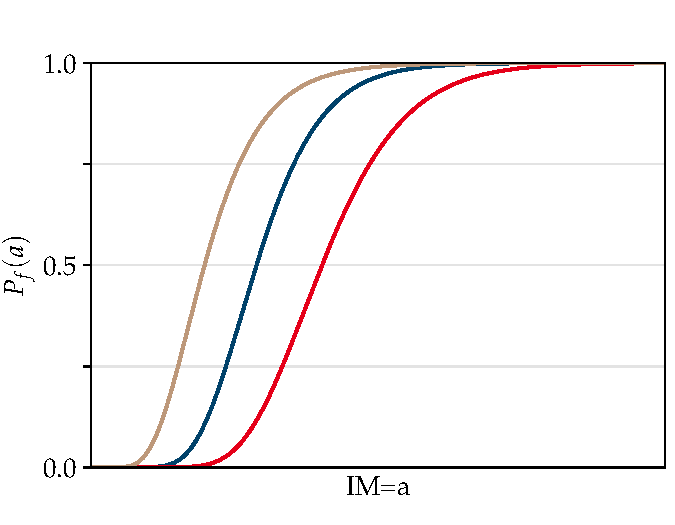
\includegraphics[width=5.225cm]{figures/intro-frags/exfrags.pdf}
    \caption{Examples of probit-lognormal fragility curves.}
    \label{fig:intro-frags:exfrags}
\end{figure}


Different strategies exist to estimate the two parameters, namely the median $\alpha$ and the log standard deviation $\beta$. Historically, maximum likelihood estimation (MLE) techniques are recommended.  %with confidence interval derivation via bootstrapping are recommended (see for instance ).
When the data are independent, the bootstrap technique can be used to obtain confidence intervals relating to the size of the sample considered (e.g. \cite{shinozuka_statistical_2000,zentner_numerical_2010,wang_influence_2020}). %, ZENTNER20101614, WangF2020}). 
% \cite{Shinozuka2000, ZENTNER20101614, WangF2020}. 
To describe this technique,
we define first the associated statistical model: the observations are modeled as realizations of the random variable $(A,Z)\in\cA\times\{0,1\}$. It is supposed that observations are independent conditionally to $\theta$ and that $(A,Z)$ are distributed conditionally to $\theta\in\Theta=(0,\infty)^2$ as:
    \begin{equation}
            A|\theta\sim A\sim H,\quad\text{and}\quad Z|A,\theta\sim\cB\left(\Phi\left(\beta^{-1}\log\frac{A}{\alpha}\right)\right),
    \end{equation}
where $H$ is the distribution of $A$ and $\cB(p)$ denotes a Bernoulli distribution of mean  $p$.
Thus, the likelihood $\ell_k$ given observations $(\mbf a^k,\mbf z^k)$ with $\mbf a^k=(a_i)_{i=1}^k$ and $\mbf z^k=(z_i)_{i=1}^{k}$ is expressed as
    \begin{equation}
        \ell_k(\mbf z^k,\mbf a^k|\theta) = \prod_{i=1}^k\ell(z_i,a_i|\theta) = \prod_{i=1}^k\Phi\left(\frac{\log a_i-\log\alpha}{\beta}\right)^{z_i}\left(1-\Phi\left(\frac{\log a_i-\log\alpha}{\beta}\right)\right)^{1-z_i}h(a_i),
    \end{equation}
where $h$ is the p.d.f. of $A$. Since the $(h(a_i))_i$ are constants of $\theta$ and are not known in general, it is common to consider the following alternative form of the likelihood:
\begin{equation}
    \ell_k(\mbf z^k|\mbf a^k,\theta) = \prod_{i=1}^k\ell(z_i|a_i,\theta) = \prod_{i=1}^k\Phi\left(\frac{\log a_i-\log\alpha}{\beta}\right)^{z_i}\left(1-\Phi\left(\frac{\log a_i-\log\alpha}{\beta}\right)\right)^{1-z_i}.
\end{equation}
The maximum likelihood estimator is $\theta^{\text{MLE}}(\mbf z^k,\mbf a^k)=\argmax_{\theta\in\Theta}\ell_k(\mbf z^k,\mbf a^k|\theta)$.
The bootstrap technique consists in deriving a stochastic estimator $\hat\theta_k^{\text{BMLE}}(\mbf z^k,\mbf a^k)$ whose distribution is defined from expressing it as: $\hat\theta^{\text{BMLE}}(\mbf z^k,\mbf a^k)=\theta^{\text{MLE}}((z_{U_i},a_{U_i})_{i=1}^k)$, where $U_1,\dots,U_k$ are i.i.d. random variables distributed w.r.t. a uniform distribution in $\{1,\dots,k\}$.



 
% we consider the statisct

% let us start by defining formally the statistical probit-lognormal model: 



\subsubsection{About the implementation of the Bayesian framework to estimate $\theta=(\alpha,\beta)$}

As a strategy that allows to estimate the parameters defining the fragility curve, 
the Bayesian framework has recently become increasingly popular in seismic fragility analysis (see e.g. \cite{gardoni_probabilistic_2002,wang_bayesian_2018,katayama_bayesian-estimation-based_2021,koutsourelakis_assessing_2010,damblin_approche_2014,tadinada_structural_2017,kwag_computationally_2018,jeon_parameterized_2019,tabandeh_physics-based_2020}). 
It is praised for its capacity to solve the irregularity issues encountered when estimating fragility curves with classical methods. For instance, the MLE-bootstrap method is known to lead to unrealistic estimates such as unit-step functions when few data are available.
However, a challenge remains when %The difficulty that remains when 
implementing the Bayesian framework, and 
lies in the selection of the prior.
As a matter of fact, as announced since \cref{chap:intro-english}, selecting a prior is a critical step in Bayesian analysis, %especially in a context where (i) the datasets of interest are light, and (ii) the methodology must be auditable.
and when exploring the literature, a wide range of different consideration can be found regarding its construction. % prior
%

%In earthquake engineering, Bayesian inference is often used to update existing log-normal fragility curves previously obtained through various approaches, assuming independent distributions for the prior values of $\alpha$ and $\beta$, such as log-normal distributions. 
%
For example, in \cite{tadinada_structural_2017} and \cite{kwag_computationally_2018}, the median prior values come from equivalent linearized mechanical models. In \cite{wang_bayesian_2018}, both aleatory and epistemic uncertainties are taken into account in the parametric model originally introduced in \cite{kennedy_probabilistic_1980}: an artificial neural network is trained and used to characterize (i) the aleatory uncertainty and (ii) the prior median value of $\alpha$, while the associated epistemic uncertainty is taken from the existing literature. The log-normal prior distribution of $\alpha$ is then updated with empirical data. 
In \cite{katayama_bayesian-estimation-based_2021}, the results of incremental dynamic analysis are used to obtain a prior value of $\alpha$, whereas the prior value of $\beta$ is determined through a parametric study. This results in satisfactory convergence, whatever its target value, before application to practical problems.
In \cite{straub_improved_2008}, the authors mainly focus on the implications for fragility analyses of statistical dependencies within the data. The prior is defined as the product of a normal distribution for $\ln(\alpha)$, and the improper distribution $1/\beta$ for $\beta$. The definition of the normal distribution is based on engineering assessments. This prior was preferred to $1/\alpha$ on the grounds that it led to unrealistically large posterior values of $\alpha$. A sensitivity analysis is further performed to examine the impact of the choice of the prior distribution on the final results.
Finally, we note that the Bayesian framework is also relevant for fitting numerical models (e.g., mathematical expressions based on engineering assessments or physics-based models) to experimental data in order to estimate fragility curves \citep{gardoni_probabilistic_2002,tabandeh_physics-based_2020} or meta-models such as logistic regressions \citep{koutsourelakis_assessing_2010,jeon_parameterized_2019}.







% In the SPRA framework, Bayesian inference is often used to update existing probit-lognormal fragility curves previously obtained through various approaches, assuming probit-lognormal distribution only for $\alpha$ \cite{WANG2018232}, 
% independent distributions for the prior values of $\alpha$ and $\beta$ such as uniform distributions \cite{KOUTSOURELAKIS2010}, the product of a normal distribution for $\ln(\alpha)$ and the improper distribution $1/\beta$ for $\beta$ \cite{Straub2008}, etc.


% in \cite{wang_bayesian_2018}, $\beta$ is replaced by in eq  to 


%\cite{Shinozuka2000,Lallemant2015,Straub2008,ZENTNER20101614, WangF2020, MANDAL201611, WANGZ2018, WANG2018232, ZHAO2020103, ELLINGWOOD2001251, KIM2004, Mai2017, TREVLOPOULOS2019,Katayama2021,LEE2023}


\section{Example of case studies}\label{sec:intro-frags:casstudies}

    \subsection{An elasto-plastic oscillator}\label{sec:intro-frags:elastoplastic}

    The first case study that we present is 
    a single-degree-of-freedom elasto-plastic oscillator with kinematic hardening.
    %It represents a con
    This simple mechanical system illustrates the essential features which can be found in the nonlinear responses of some real-world structures under seismic excitation and has, for this reason, already been used in several studies \citep{trevlopoulos_parametric_2019,sainct_efficient_2020,gauchy_importance_2021}.
    In addition, it provides reference results as a reasonable numerical cost.
    It is depicted in \cref{fig:intro-frags:elasto}, and
    its equation of motion when submitted to an excitation $s$ is the following:
    \begin{equation}
        x''(t) +2\xi2\pi f_L x'(t)+f^{\text{nl}}(t) = -s(t),
    % \ddot{y}(t) + 2 \zeta \omega_{\text{L}}\dot{y}(t) + f(t) = -s(t) \ ,
    \end{equation}
    %with $s(t)$ a seismic signal, $\dot{y}(t)$ and $\ddot{y}(t)$ respectively the relative velocity and acceleration of the mass, 
    with $x''$ and $x'$ respectively the relative  acceleration and velocity of the mass,  $\xi$ the damping ratio, $f_L$ the circular frequency, and $f^{\text{nl}}$ the nonlinear resisting force.

    \begin{figure}[h]
        \centering
        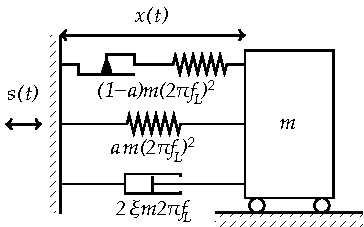
\includegraphics[width=5.5cm]{figures/intro-frags/KBEPO_rheo.pdf}
        \caption{Elasto-plastic oscillator of mass $m$ with kinematic hardening, with parameters $f_{\text{L}} = 5$ Hz and $\xi = 2\%$. The yield limit is $Y = 5.10^{-3}$~m, and the post-yield stiffness is $20\%$ of the elastic stiffness, i.e., $a = 0.2$.} 
        \label{fig:intro-frags:elasto}  
    \end{figure}

    
    
    The relevant EDP is the absolute maximum value of the mass’ displacement, i.e., $\text{EDP}=\max_{t\in [0, T]}|x(t)|$, where $T$ is the duration of the seismic excitation. In \cref{fig:intro-frags:oscillclouds}, we plot that EDP that has been derived for the $10^5$ seismic signals generated and presented in \cref{sec:intro-frags:data}.

    \begin{figure}[h]
        \centering
        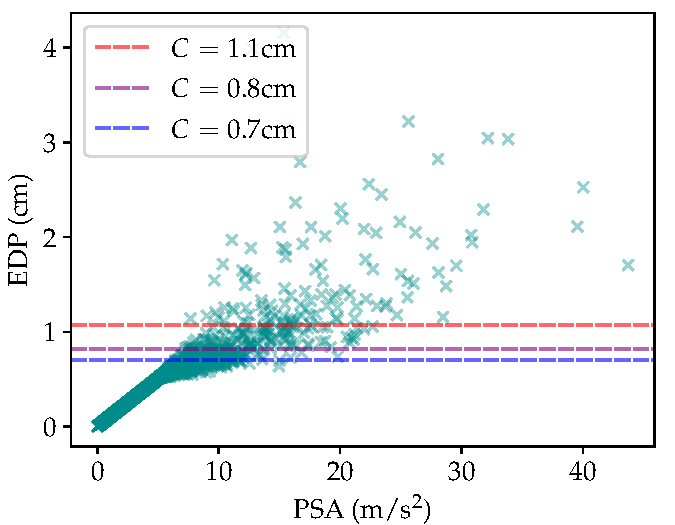
\includegraphics[width=5cm]{figures/intro-frags/oscill/cloudPSA.pdf}
        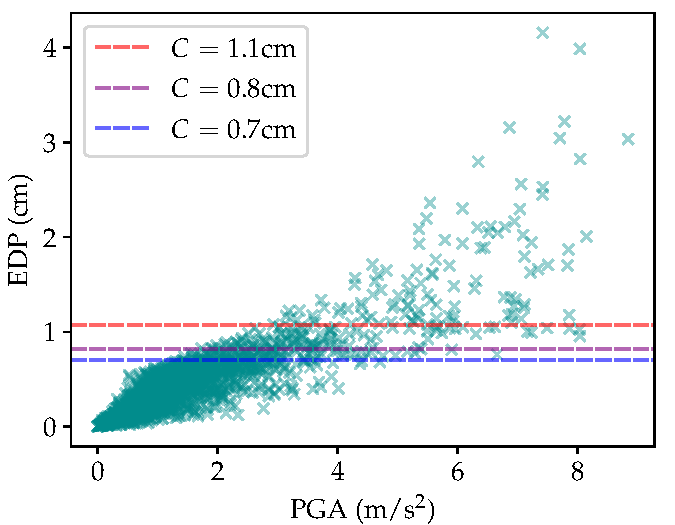
\includegraphics[width=5cm]{figures/intro-frags/oscill/cloudPGA.pdf}
        \caption{Results of the $10^5$ simulations conducted on the elasto-plastic oscillator. Each cross is an element of the dataset (IM, EDP) where the IM is the PSA (left) and the PGA (right). Different critical rotation thresholds $C$ are plotted in dashed lines. They yield different proportions of failures in the dataset: respectively 95$\%$ (red), $90\%$ (purple) and $85\%$ (blue).}
        \label{fig:intro-frags:oscillclouds}
    \end{figure}


    Since a very large number of data are available for this case study, it is possible to derive a reference fragility curve using the non-parametric method that is described in \cref{sec:intro-frags:subsec-nonparametric}.
    Such reference fragility curves are plotted in \cref{fig:intro-frags:oscillrefs}, for different thresholds $ C $ that define the failure.
    In general, the failure criterion that corresponds to the $90\%$-level quantile of the maximum displacements calculated with the $10^5$ artificial signals is chosen, i.e., $C = 8.0 \; 10^{-3}$~m.
    The reference 
    curves are compared with the probit-lognormal fragility curves (described in \cref{sec:intro-frags:subsec-parametric}) where $\theta$ is estimated by MLE using the full dataset as well. This comparison is presented for both the PSA and the PGA as IM.
    It demonstrates that the probit-lognormal model allows a good approximation of the reference curve for this case study.

    \begin{figure}[h]
        \centering
        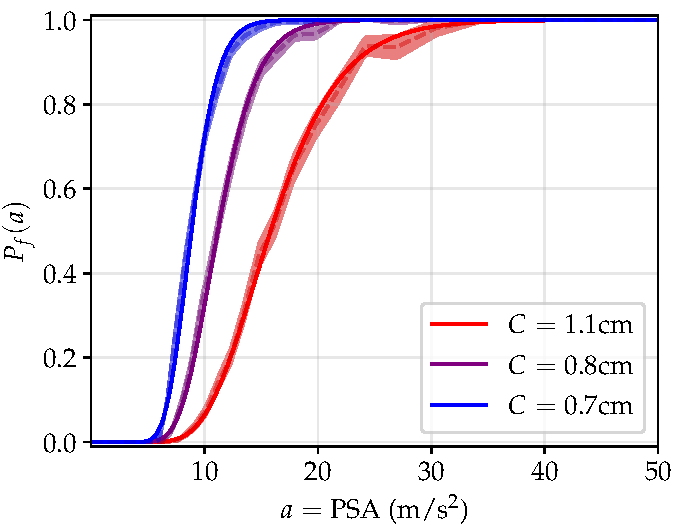
\includegraphics[width=5cm]{figures/intro-frags/oscill/refs_PSA.pdf}
        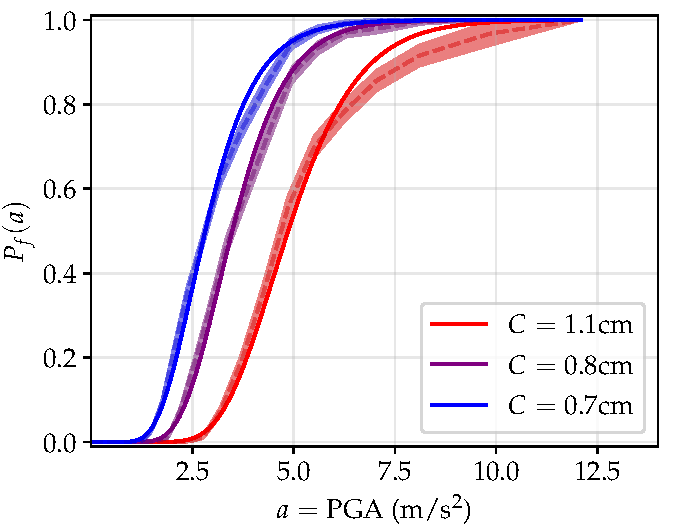
\includegraphics[width=5cm]{figures/intro-frags/oscill/refs_PGA.pdf}
        \caption{{Reference non-parametric fragility curves of the elasto-plastic oscillator obtained via Monte Carlo estimates (dashed lines) surrounded by their $95\%$ confidence intervals, for different critical displacement threshold $C$ with (left) the PSA and (right) the PGA as IM.} The thresholds yield different proportions of failures in the dataset: respectively $95\%$ (red), $90\%$ (purple) and $85\%$ (blue).
        For each value of $C$ are plotted (same color, solid line) the corresponding probit-lognormal MLE.}
        \label{fig:intro-frags:oscillrefs}
    \end{figure}


    
    \subsection{A piping system from a pressurized water reactor}\label{sec:intro-frags:piping}

    {The case study presented in this section is a piping system that was tested on the Azalee shaking table at the EMSI laboratory of CEA/Saclay, as shown in \cref{fig:ASG}-left. \Cref{fig:ASG}-right depicts the finite element model (FEM), based on beam elements and implemented through the proprietary FE code CAST3M \citep{cea_cast3m_2019}. The validation of the FEM was carried out thanks to an experimental campaign described in \cite{touboul_seismic_1999}.}

    The mock-up comprises a carbon steel TU42C pipe with an outer diameter of 114.3 mm, a thickness of 8.56 mm, and a 0.47 elbow characteristic parameter. This pipe, filled with water without pressure, includes three elbows, with a valve-mimicking mass of 120 kg, constituting over 30\% of the mock-up's total mass. One end of the mock-up is clamped, while the other is guided to restrict displacements in the X and Y directions. Additionally, a rod is positioned atop the specimen to limit mass displacements in the Z direction (refer to \cref{fig:ASG}-right). During testing, excitation was applied exclusively in the X direction.



\begin{figure}[h]
		\centering		
		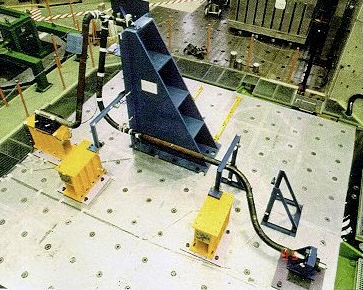
\includegraphics[width=5.2cm]{figures/intro-frags/ASG.jpg}
		\hspace{1cm}
		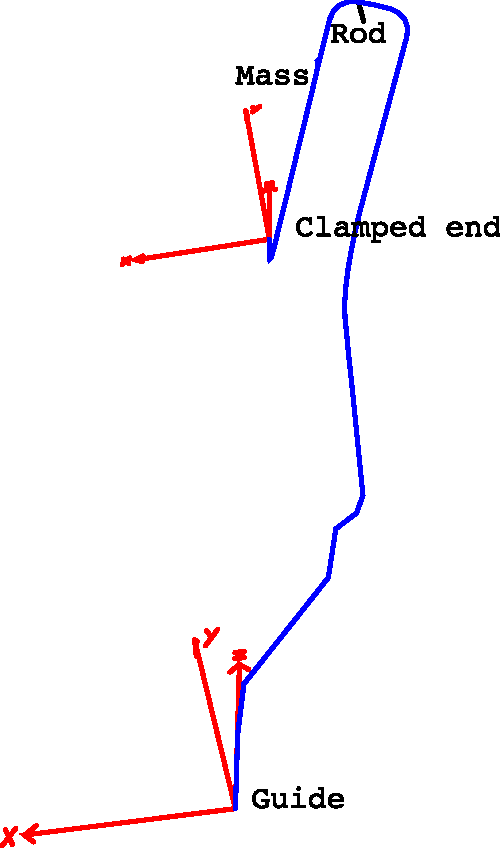
\includegraphics[width=2.5cm]{figures/intro-frags/ASG_FEM.pdf}
		\caption{(left) Overview of the piping system ---which is part of a French pressurized water reactor--- on the Azalee shaking table and (right) associated finite element model.}
		\label{fig:ASG}
	\end{figure}




    {In order to conduct comparative performance studies, numerous simulations have been performed. They were carried out from a subset of $8\cdot10^4$ of the $10^5$ artificial seismic signals. Nevertheless, as in practice the piping system is located in a building, the artificial signals were filtered using a fictitious 2\% damped linear single-mode building at 5 Hz, which corresponds to the first eigenfrequency of the 1\% damped piping system.  In such a situation, for some seismic signals, the behavior of the piping system is nonlinear. Regarding the nonlinear constitutive law of the material, a bilinear law exhibiting kinematic hardening was used to reproduce the overall nonlinear behavior of the mock-up with satisfactory agreement compared to the results of the seismic tests \citep{touboul_seismic_1999}. Following the recommendation in \cite{touboul_enhanced_2006}, we consider that the engineering demand parameter (EDP) is the out-of-plane rotation of the elbow near the clamped end of the mock-up. As a result we have a dataset of $8\cdot10^4$ independent tuples of the form (IM, EDP) for different IMs. In \cref{fig:asg:scattersIMs} are plotted the elements of the datasets (PSA, EDP) and (PGA, EDP), along with different critical thresholds.}
    %The binary data are defined from the condition that failure happens when the EDP is larger than the threshold value.}

    \begin{figure}[h]
        \centering%
        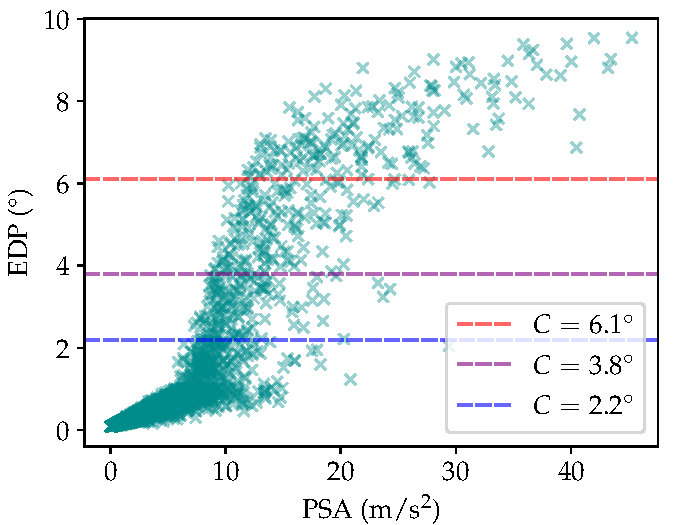
\includegraphics[width=5cm]{figures/intro-frags/asg/cloud_PSA_light.pdf}%
        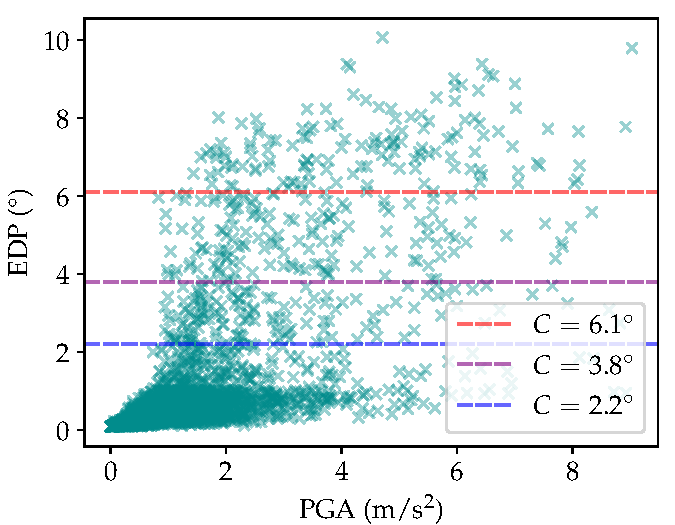
\includegraphics[width=5cm]{figures/intro-frags/asg/cloud_PGA_light.pdf}%
        \caption{Results of the $8\cdot10^4$ numerical simulations conducted on the piping system. Each cross is an element of the dataset (IM, EDP) where the IM is the PSA (left) and the PGA (right). Different critical rotation thresholds $C$ are plotted in dashed lines. They yield different proportions of failures in the dataset: respectively 95$\%$ (red), $90\%$ (purple) and $85\%$ (blue).}
        \label{fig:asg:scattersIMs}
        \end{figure}
    
    The complete set of $8\cdot 10^4$ simulations provides a satisfactory dataset to derive a reference of the seismic fragility curve for this case study, still using the non-parametric method depicted in \cref{sec:intro-frags:subsec-nonparametric}.
    % In 
    In \cref{fig:asg:reference-frags}, we compare this non-parametric reference with the parametric fragility curve using the probit-lognormal model (\cref{sec:intro-frags:subsec-parametric}) where $\alpha$ and $\beta$ are estimated by MLE using the $8\cdot 10^4$ data items as well. {This comparison is presented considering different critical rotation thresholds $ C $ of the equipment for both the PSA and the PGA. First, it should be noted that, with the PGA as IM, it is not possible to completely describe the fragility curve. For the maximum PGA values observed, the failure probabilities stagnate between 0.5 and 0.8 depending on the failure criterion considered. Therefore, the PGA is not the most suitable IM of the two. For the type of structure considered here, this point is well documented in the literature. Then, the comparisons demonstrate, in our setting, the adequacy of a probit-lognormal modeling of the fragility curves, even with high failure thresholds.} Its bias with non-parametric fragility curve exists but remains limited. When the number of observations is small, this model bias is negligible in front of the uncertainty on the estimates.


    
    
    \begin{figure}[h]
        \centering
        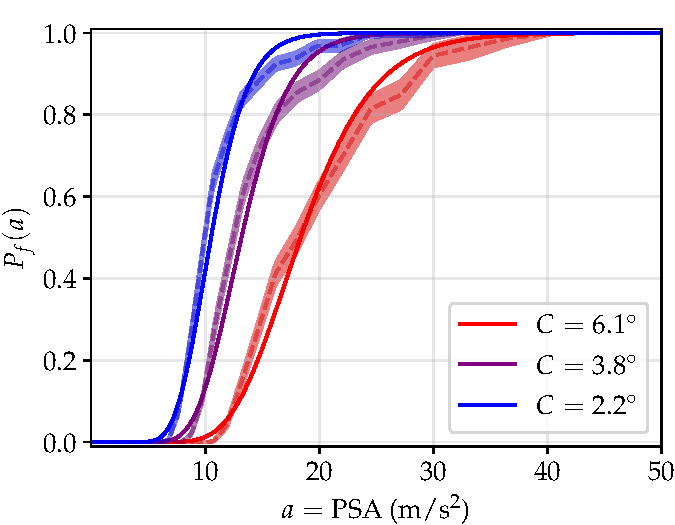
\includegraphics[width=5cm]{figures/intro-frags/asg/refs_PSA.pdf}
        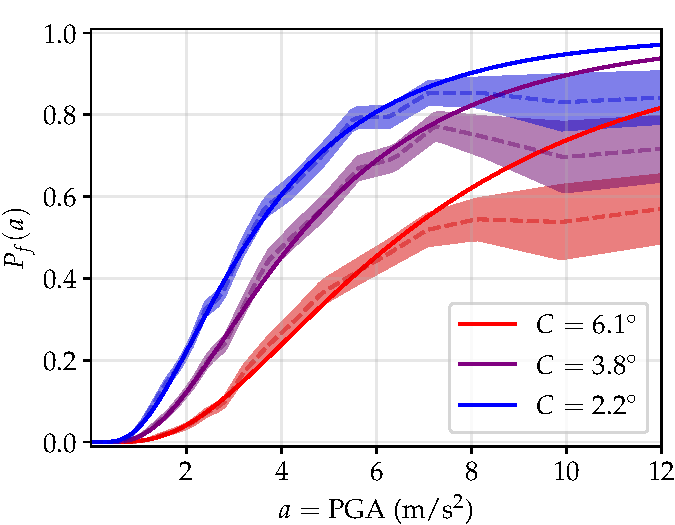
\includegraphics[width=5cm]{figures/intro-frags/asg/refs_PGA.pdf}
        \caption{{Reference non-parametric fragility curves of the piping system obtained via Monte Carlo estimates (dashed lines) surrounded by their $95\%$ confidence intervals, for different critical rotation threshold $C$ with (left) the PSA and (right) the PGA as IM.} The thresholds yield different proportions of failures in the dataset: respectively $95\%$ (red), $90\%$ (purple) and $85\%$ (blue).
        For each value of $C$ are plotted (same color, solid line) the corresponding probit-lognormal MLE.}
        \label{fig:asg:reference-frags}
        \end{figure}

    
    %The others serve the illustration.
    %These values are turned into binary outcomes ---failures or successes--- depending on them exceeding a critical threshold. 
    %Response here corresponds to the binary outcome: failure or success.

  
   
    


    \subsection{Stacked structure for storage of packages}\label{sec:intro-frags:stacked}

% \cite{beylat_contribution_2020}
    % \subsection{Appropriate modeling with how many data and what data}


    The case study considered hereafter concerns a freestanding stacked structure composed of three pallets intended for the storage of packages. As shown in \cref{fig:intro-frags:EDEN}, it is a square-based structure 3 meters high with a slenderness of 2.4.
    
    
    
    The mass of one package is equal to 265~kg, whereas the mass of one pallet is equal to 60 kg. The total mass of the structure is equal to $3,360$~kg. The pallets are made of 3~mm-thick hollow-section aluminum square tubes. These tubes are welded and form the base and uprights of the pallets. The base of a pallet supports four freestanding packages, whereas the uprights support the upper freestanding pallet(s). The stacked structure was studied in \cite{beylat_contribution_2020} by means, among others, of a complete experimental campaign, which was carried out on the 1D shaking table ``Vesuve'' of CEA/Saclay. In particular, the stack was subjected to 21 of the 97 real signals that were used to fit the generator depicted in \cref{sec:intro-frags:data}.
    For this structure, the EDP corresponds to the maximal displacement of the top of the stack.
    % the failure criterion relates to an excessive displacement. %of the top of the stack. 
    An example of a test result is shown in \cref{fig:intro-frags:EDEN}, which depicts the horizontal displacements over time of the top of the stack. The initial position is indicated in red, while the different positions in time are indicated in blue. {Due to uplift, sliding, and rotation motions, the top of the stack exceeds, for 2 of the 21 tests, the admissibility criterion, which is materialized in black. }
    Only a little number of experimental results are available for this case study, so that it is not possible to derive a reference fragility curve here.





    \begin{figure}[h]
		\centering		
		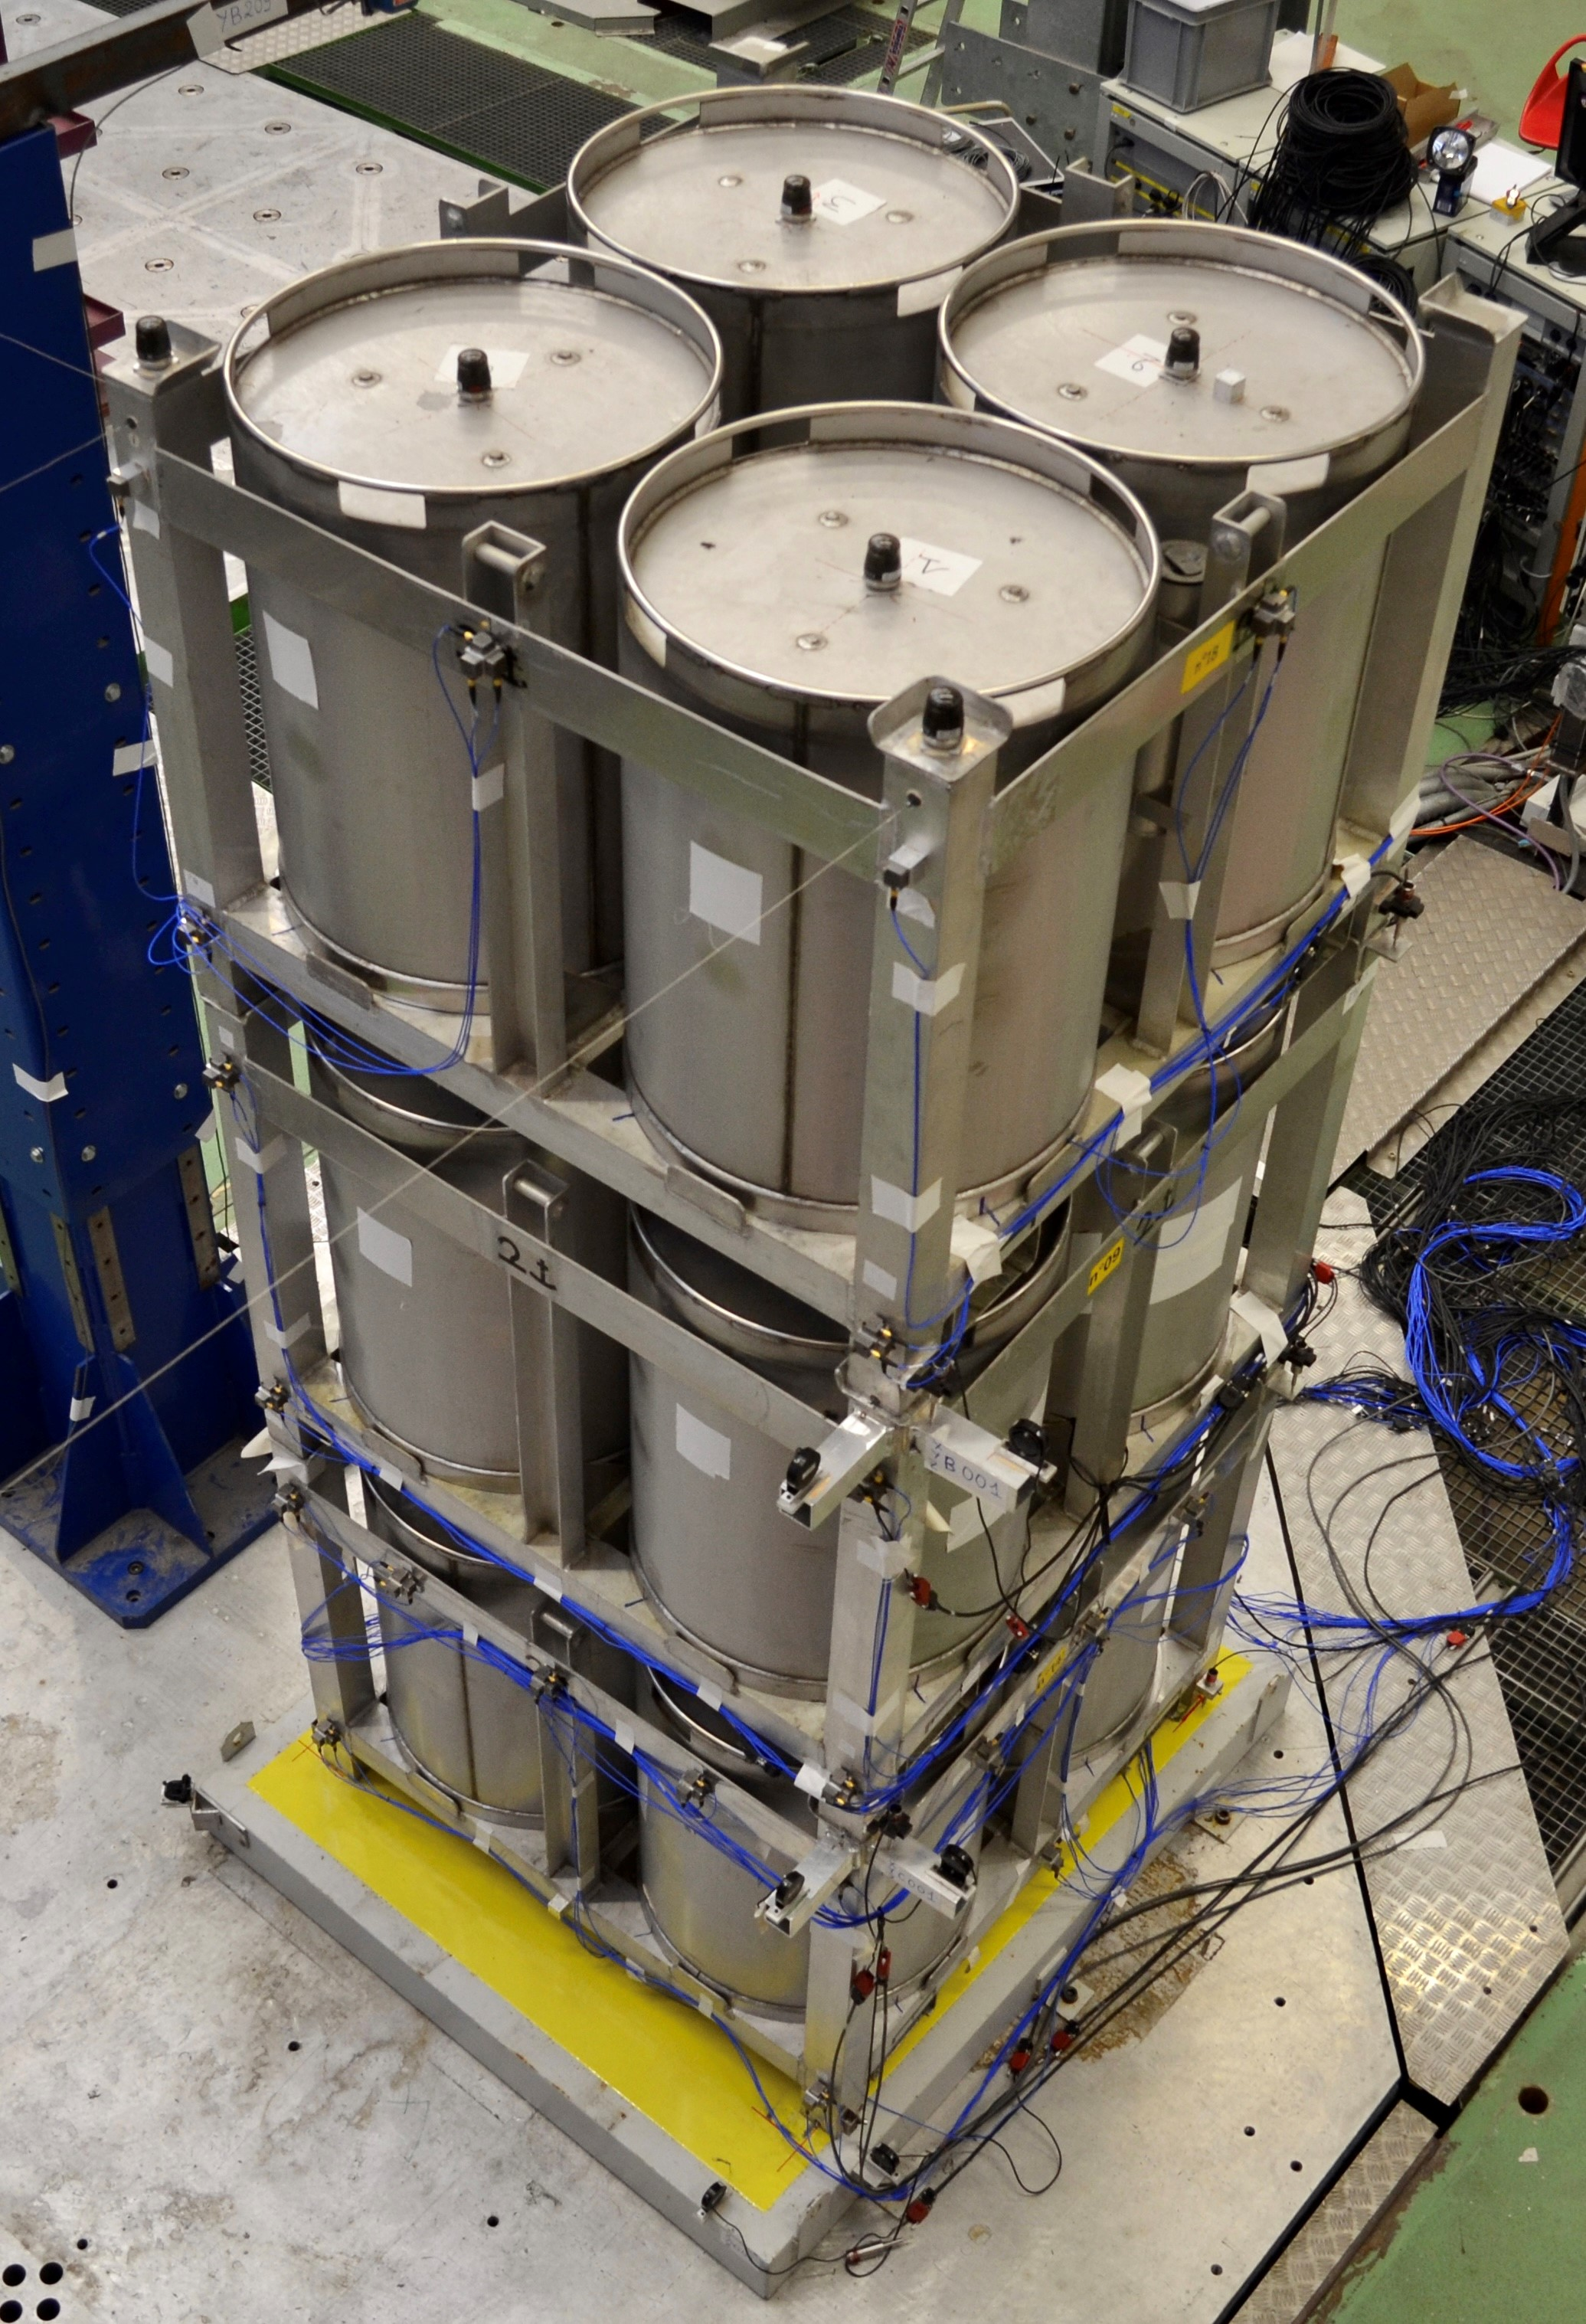
\includegraphics[width=4.5cm]{figures/intro-frags/EDEN.jpg}
		\hspace{0.5cm}
		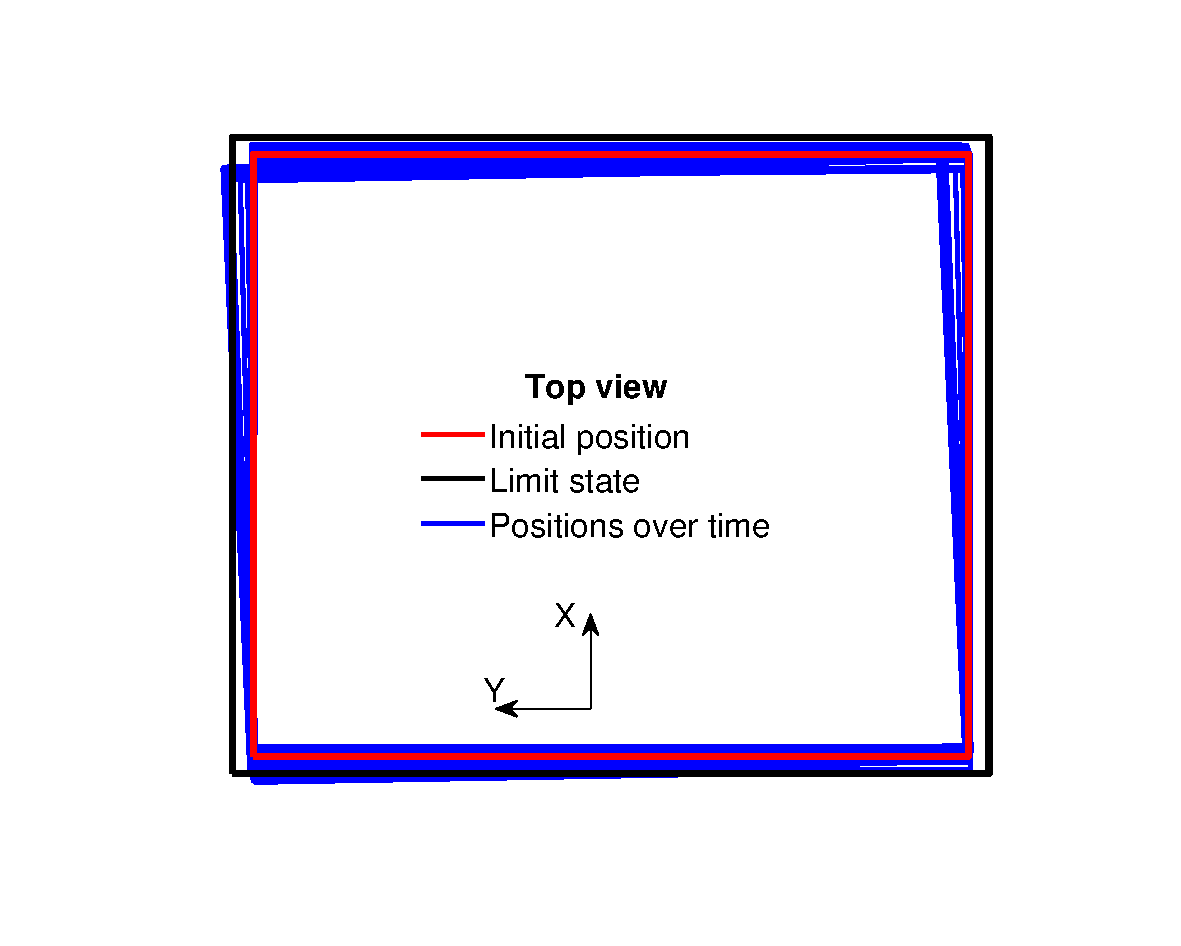
\includegraphics[width=7cm]{figures/intro-frags/EDEN_R169.pdf}
		\caption{(left) Overview of the stacked structure placed on the Vesuve 1D shaking table and (right) example of test result: horizontal displacements of the top of the stack when subjected to seismic excitation in the X direction.}
		\label{fig:intro-frags:EDEN}
	\end{figure}  


\section{Conclusion: which case study and which data for a Bayesian estimation of fragility curves?}\label{sec:intro-frags:conclusion}

% The estimation of seismic fragility curves is an open question that is 


In the literature, many works address the estimation of seismic fragility curves, introducing many approaches to handle that task.
Nevertheless, the appropriate method to provide robust estimates heavily depends on the characteristics of the studied equipments, on the 
type of data that are available, and on their number.
% As a matter of fact, we have cited numerou
% The data curation is itself a main step that has to be taken into account when conducting a methodology of seismic fragility curves estimation. 
In this chapter, we have described standard forms of datasets considered in the literature, and we have depicted how they are used to providing approximations of fragility curves using different approaches.

In the worst case, the dataset is %, limiting the use of non-parametric methods
%and 
made of tuples composed by (i) a value of the IM, and (ii) a binary outcome about the system's response: failure or non-failure.
In those cases, the non-parametric models provide limited estimations, and a parametric model, such as the prominent probit-lognormal one has to be favored.
If the dataset is also scarce, then most classical frequentist methods become unsatisfying as well, letting the Bayesian framework to arise as a cornerstone.
% leading to 

However, 
a major issue connects all the studies 
% while a plethora of studies 
suggesting a Bayesian estimation of seismic fragility curves that we reviewed: the prior selection is not thoroughly questioned. Moreover, the choices done regarding its construction are hard to justify, and one could question the reliability of the provided estimates.
% , we observed
% they all suffer from their prior choice, 

% questionable priors
% choices

%when reviewing the literature, we observed that 

All in all, this chapter and that last thought introduce the essential interplay that exists between the \cref{part:ref-theory} and \cref{part:spra} of this manuscript.
Since our work is sought to be applied on case studies taken from the nuclear industry, we aim at providing a reliable and auditable methodology when we estimate seismic fragility curves.
The expected  auditability also concerns the choice of the prior, which hence must be constructed in a way that ensures its objectivity.





\newpage
\thispagestyle{plain}






% In this case, a paramterized model is prominent







% We have described 







% \section{Conclusion}



